\documentclass{beamer}
\let\Tiny=\tiny
\usepackage[utf8]{inputenc}
\RequirePackage[ngerman]{babel}%
\RequirePackage[T1]{fontenc}%
\usepackage[babel,german=quotes]{csquotes}
\usepackage{eurosym}%
\usepackage{booktabs}
\usepackage{tabu}
\usepackage{colortbl}
\usepackage{xcolor}
%\usetheme[height=7mm]{Rochester}
%\usetheme{Antibes}
\usetheme{Copenhagen}
\usecolortheme{dolphin}
%\useoutertheme{infolines} 
\title[Concurrent C Programming]{TCP File Server}
\author{Cristoffel Gehring}
\institute{ZHAW}
\date{\today}
\begin{document}
\begin{frame}
  \titlepage
  \centering
  
\includegraphics[width=0.2\textwidth]{./pics/zhaw.png}
\end{frame}

\begin{frame}
  \tableofcontents
\end{frame}

\section{Vorgehen}
\begin{frame}
  \frametitle{Vorgehen}
  \begin{center}
	\begin{itemize}
	  \item Recherche und Planung vor Pfingsten
	  \item Intensivphase 3 Tage über Pfingsten 
	  \item Jeder Tag ein Deliverable
	  \item Modularer Aufbau
	\end{itemize}
  \end{center}
\end{frame}

\section{Implementierung}
\begin{frame}
  \frametitle{POSIX named Shared Memory für jede Datei}
  \begin{itemize}
	\item Shared Memory Segment wird nach '\\Dateiname' benannt 
	\item Platz für char[length] wird angelegt
  \end{itemize}
\end{frame}

\begin{frame}
  \frametitle{Seperates Shared Memory für Dateiliste}
  \begin{itemize}
	\item char[maxDateien][maxNameLength]
	\item Alle Dateien bekommen einen Eintrag
	\item Muss laufend aktualisiert werden
	\item Muss mit Sempaphore geschützt werden
  \end{itemize}
\end{frame}

\begin{frame}
  \frametitle{Semaphoren}
  \begin{itemize}
	\item POSIX named Semaphore
	\item Jede Datei bekommt zwei Semaphore\\
	  read: '\\Dateiname_r' oder\\
	  write: '\\Dateiname_w'
	\item Semaphore wird nach  benannt 
	\item Anzahlt Leser wird gezählt.\\
	  Falls 0, kann geschrieben werden
  \end{itemize}

\end{frame}

%\section{System Call Rootkit}
%\begin{frame}
%  \centering
%  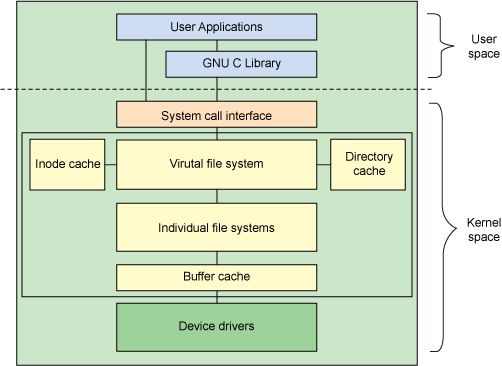
\includegraphics[height=0.9\textheight]{./pics/linux_arch}
%\end{frame}
%
%\section{VFS Rootkit}
%\begin{frame}
%  \centering
%  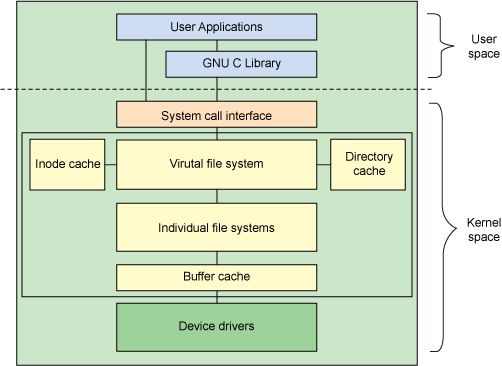
\includegraphics[height=0.9\textheight]{./pics/linux_arch}
%\end{frame}
%
%%\begin{frame}
%%  \frametitle{Lösungsansatz für die Probleme}
%%  \begin{itemize}
%%	\item Velos verteilen sich ungleichmässig\\
%%	  $\hookrightarrow$ Cleveres Accounting-System
%%	\item Vandalismus\\
%%	  $\hookrightarrow$ Benutzer muss ein verifiziertes Konto anlegen\\
%%	  $\hookrightarrow$ Bewegungs- und Reifendrucksensor am Velo
%%	\item Komplizierte Ausleihen\\
%%	  $\hookrightarrow$ Konto kann online angelegt werden 
%%  \end{itemize}
%%\end{frame}
%%
%%\section{Spezifikation <<öIv>>}
%%\begin{frame}
%%  \centering
%%  \frametitle{Spezifikation}
%%  \includegraphics[height=0.9\textheight]{./pics/schema.png}
%%\end{frame}
%%
%%\begin{frame}
%%  \frametitle{Client Applikation}
%%  \begin{minipage}{0.50\textwidth}
%%	\begin{center}
%%	  \includegraphics[width=0.5\textwidth]{./pics/schemaClient.png}
%%	\end{center}
%%  \end{minipage}
%%  \begin{minipage}{0.4\textwidth}
%%	\begin{itemize}
%%	  \item Bedienbar auf allen internetfähigen Geräten
%%	  \item Kunden können Kundenkonto erstellen
%%	  \item Velos können in Echtzeit geortet, reserviert und freigegeben werden
%%	\end{itemize}
%%  \end{minipage}
%%\end{frame}
%%
%%\begin{frame}
%%  \frametitle{Velos}
%%  \begin{minipage}{0.5\textwidth}
%%	\begin{center}
%%	  \includegraphics[width=0.5\textwidth]{./pics/schemaVelo.png}
%%	\end{center}
%%  \end{minipage}
%%  \begin{minipage}{0.4\textwidth}
%%	\begin{itemize}
%%	  \item Bestimmen eigene Position über GPS
%%	  \item Kommunizieren über GPS/GPRS mit dem Back-End
%%	  \item Haben 4 Stati (frei, belegt, reserviert, beschädigt)
%%	  \item Können eigenen Zustand messen und in den Status beschädigt
%%	\end{itemize}
%%  \end{minipage}
%%\end{frame}
%%
%%\begin{frame}
%%  \frametitle{Backend}
%%  \begin{minipage}{0.5\textwidth}
%%	\begin{center}
%%	  \includegraphics[width=0.5\textwidth]{./pics/schemaBackend.png}
%%	\end{center}
%%  \end{minipage}
%%  \begin{minipage}{0.4\textwidth}
%%	\begin{itemize}
%%		\item Sammelt Postitionen der Velos und überprüft deren Status
%%		\item Errechnet daraus ein Angebot
%%		\item Bedient Anfragen der Clients
%%		\item Kann 3 Stati setzen (frei, belegt, reserviert)
%%	\end{itemize}
%%  \end{minipage}
%%\end{frame}
%%
%%\section{Technische Realisierung}
%%\begin{frame}
%%  \frametitle{Technische Realisierung}
%%  \begin{itemize}
%%	\item Back-End / Client\\
%%	  $\hookrightarrow$ MVC\\
%%	  $\hookrightarrow$ PaaS (Platform as a Service)
%%	\item Boardrechner des Velos\\
%%	  $\hookrightarrow$ Atmel AVR
%%	\item Elektronische Zustandsüberwachung\\
%%	  $\hookrightarrow$ Reifendruck-Sensor\\
%%	  $\hookrightarrow$ Bewegungs-Sensor
%%  \end{itemize}
%%\end{frame}
%%
%%\section{Fazit}
%%\begin{frame}
%%  \frametitle{Fazit}
%%  Knackpunkte
%%  \begin{itemize}
%%	\item Cleveres Accounting-Konzept
%%	\item Realisierung der Back-End SW
%%	\item Entwicklung der Velo-Elektronik
%%  \end{itemize}
%%  Fragezeichen
%%  \begin{itemize}
%%	\item Authentifizierung der neuen Benutzer
%%	\item Bezahlungsart 
%%  \end{itemize}
%%  Nächste Schritte
%%  \begin{itemize}
%%	\item Weltweit Systeme testen
%%	\item GPS Chip mit AVR-Mikontroller ansteuern\\
%%	  $\hookrightarrow$ Seminar: Concurrent Programming in C
%%  \end{itemize}
%%\end{frame}
%\end{document}
